
\textcolor{red}{Should be add a background section here present problem formulation?}

\section{Methods}
% TODO(drafting note, not for the paper): pdcm_theory is good for an appendix
% section, but it is not well-organized or well-motivated enough for the main
% text. This section is the new, better-motivated outline.

\textbf{1.} Given a sampling distribution
\[
    p_t=(p_{t,1},\ldots,p_{t,K})\in
    \DeltaK
    \coloneqq
    \left\{p\in\R_+^K:\sum_{k=1}^K p_k=1\right\}.
\]
By performance difference lemma~\citep{Kakade2002ApproximatelyOA},
the \textit{policy improvement} of task $k$ is
\begin{equation}
\label{eq:policy_improvement_is}
U_{t, k}(p_t)
\coloneqq
J(\pi_{t+1}) - J(\pi_t) = 
\mathbb{E}_{x\sim \mathcal{X}_k} \left[
\mathbb{E}_{y\sim \pi_t(\cdot\mid x)}
\left[
\frac{\pi_{t+1}(y\mid x)}
{\pi_{t}(y\mid x)}
A_{\pi_{t}}(y\mid x)
\right]\right],
\end{equation}
where $\mathcal{X}_k$ is the input space for task $k$ and $\pi_{t+1}$ is the one-step improved policy with respect to the sampling distribution $p_t$.
The goal of non-asymptotic RL post-training is to maximize the total
policy improvement over $T$ iterations:
\begin{equation}
    \max_{p_t \in \Delta_K}J(\pi_T) - J(\pi_0) = \max_{p_t \in \Delta_K} \sum_{t=0}^{T-1} U_t(p_t),
\end{equation}
where $U_t(p_t) = \sum_{k = 1}^K U_{t, k}(p_t)$. However, maximizing the total policy improvement can lead to skewed development
over tasks that should otherwise be treated equally. To address this, 
we introduce the following constraint that no task should be left behind
what would be achieved by a uniform allocation $u = (\frac{1}{K},\ldots,\frac{1}{K})$ by a threshold $\epsilon>0$:
\begin{equation} \label{eq:constraint_uniform_baseline}
\sum_{t = 1}^T U_{t, k}\left( u \right) - U_{t, k}(p_t) \leq \epsilon, \quad \forall k\in[K].
\end{equation}
In practice, it is cost-prohibitive to estimate 
$U_{t, k}\left( u \right)$, as it involves computing the
counterfactual policy improvement of a uniform baseline. Recent work~\citep{datamixinglaws2024,aioli2025,autoscale2025} suggests that the policy-improvement surface with respect to mixture allocation is approximately concave along linear interpolation paths. We take this as our standing assumption.
\begin{assumption}[Directional concavity of task response]
\label{asm:concavity}
For every task $k\in[K]$ and iteration $t$, the task-wise utility $U_{t,k}$ admits a
supergradient $g_{t,k}=\nabla U_{t,k}(p_t)$ with respect to the sampling distribution
$p_t$, so that
\begin{equation} \label{eq:constraint_upper_bound}
U_{t, k}\left( u \right) - U_{t, k}(p_t) \leq \langle g_{t, k}, u - p_t \rangle .
\end{equation}
\end{assumption}
\Cref{eq:constraint_uniform_baseline} would be satisfied if we instead impose the RHS of \Cref{eq:constraint_upper_bound}, albeit being a more conservative constraint. This leads to the following constrained optimization problem:
\begin{equation} \label{eq:constrained_optimization_problem}
\begin{aligned}
\max_{p_t \in \Delta_K} & \quad \sum_{t=0}^{T-1} U_t(p_t) \\
\text{s.t.} & \quad \sum_{t = 1}^T \langle g_{t, k}, u - p_t \rangle \leq \epsilon, \quad \forall k\in[K], \forall t\in[T].
\end{aligned}
\end{equation}

\begin{figure*}
    \centering
    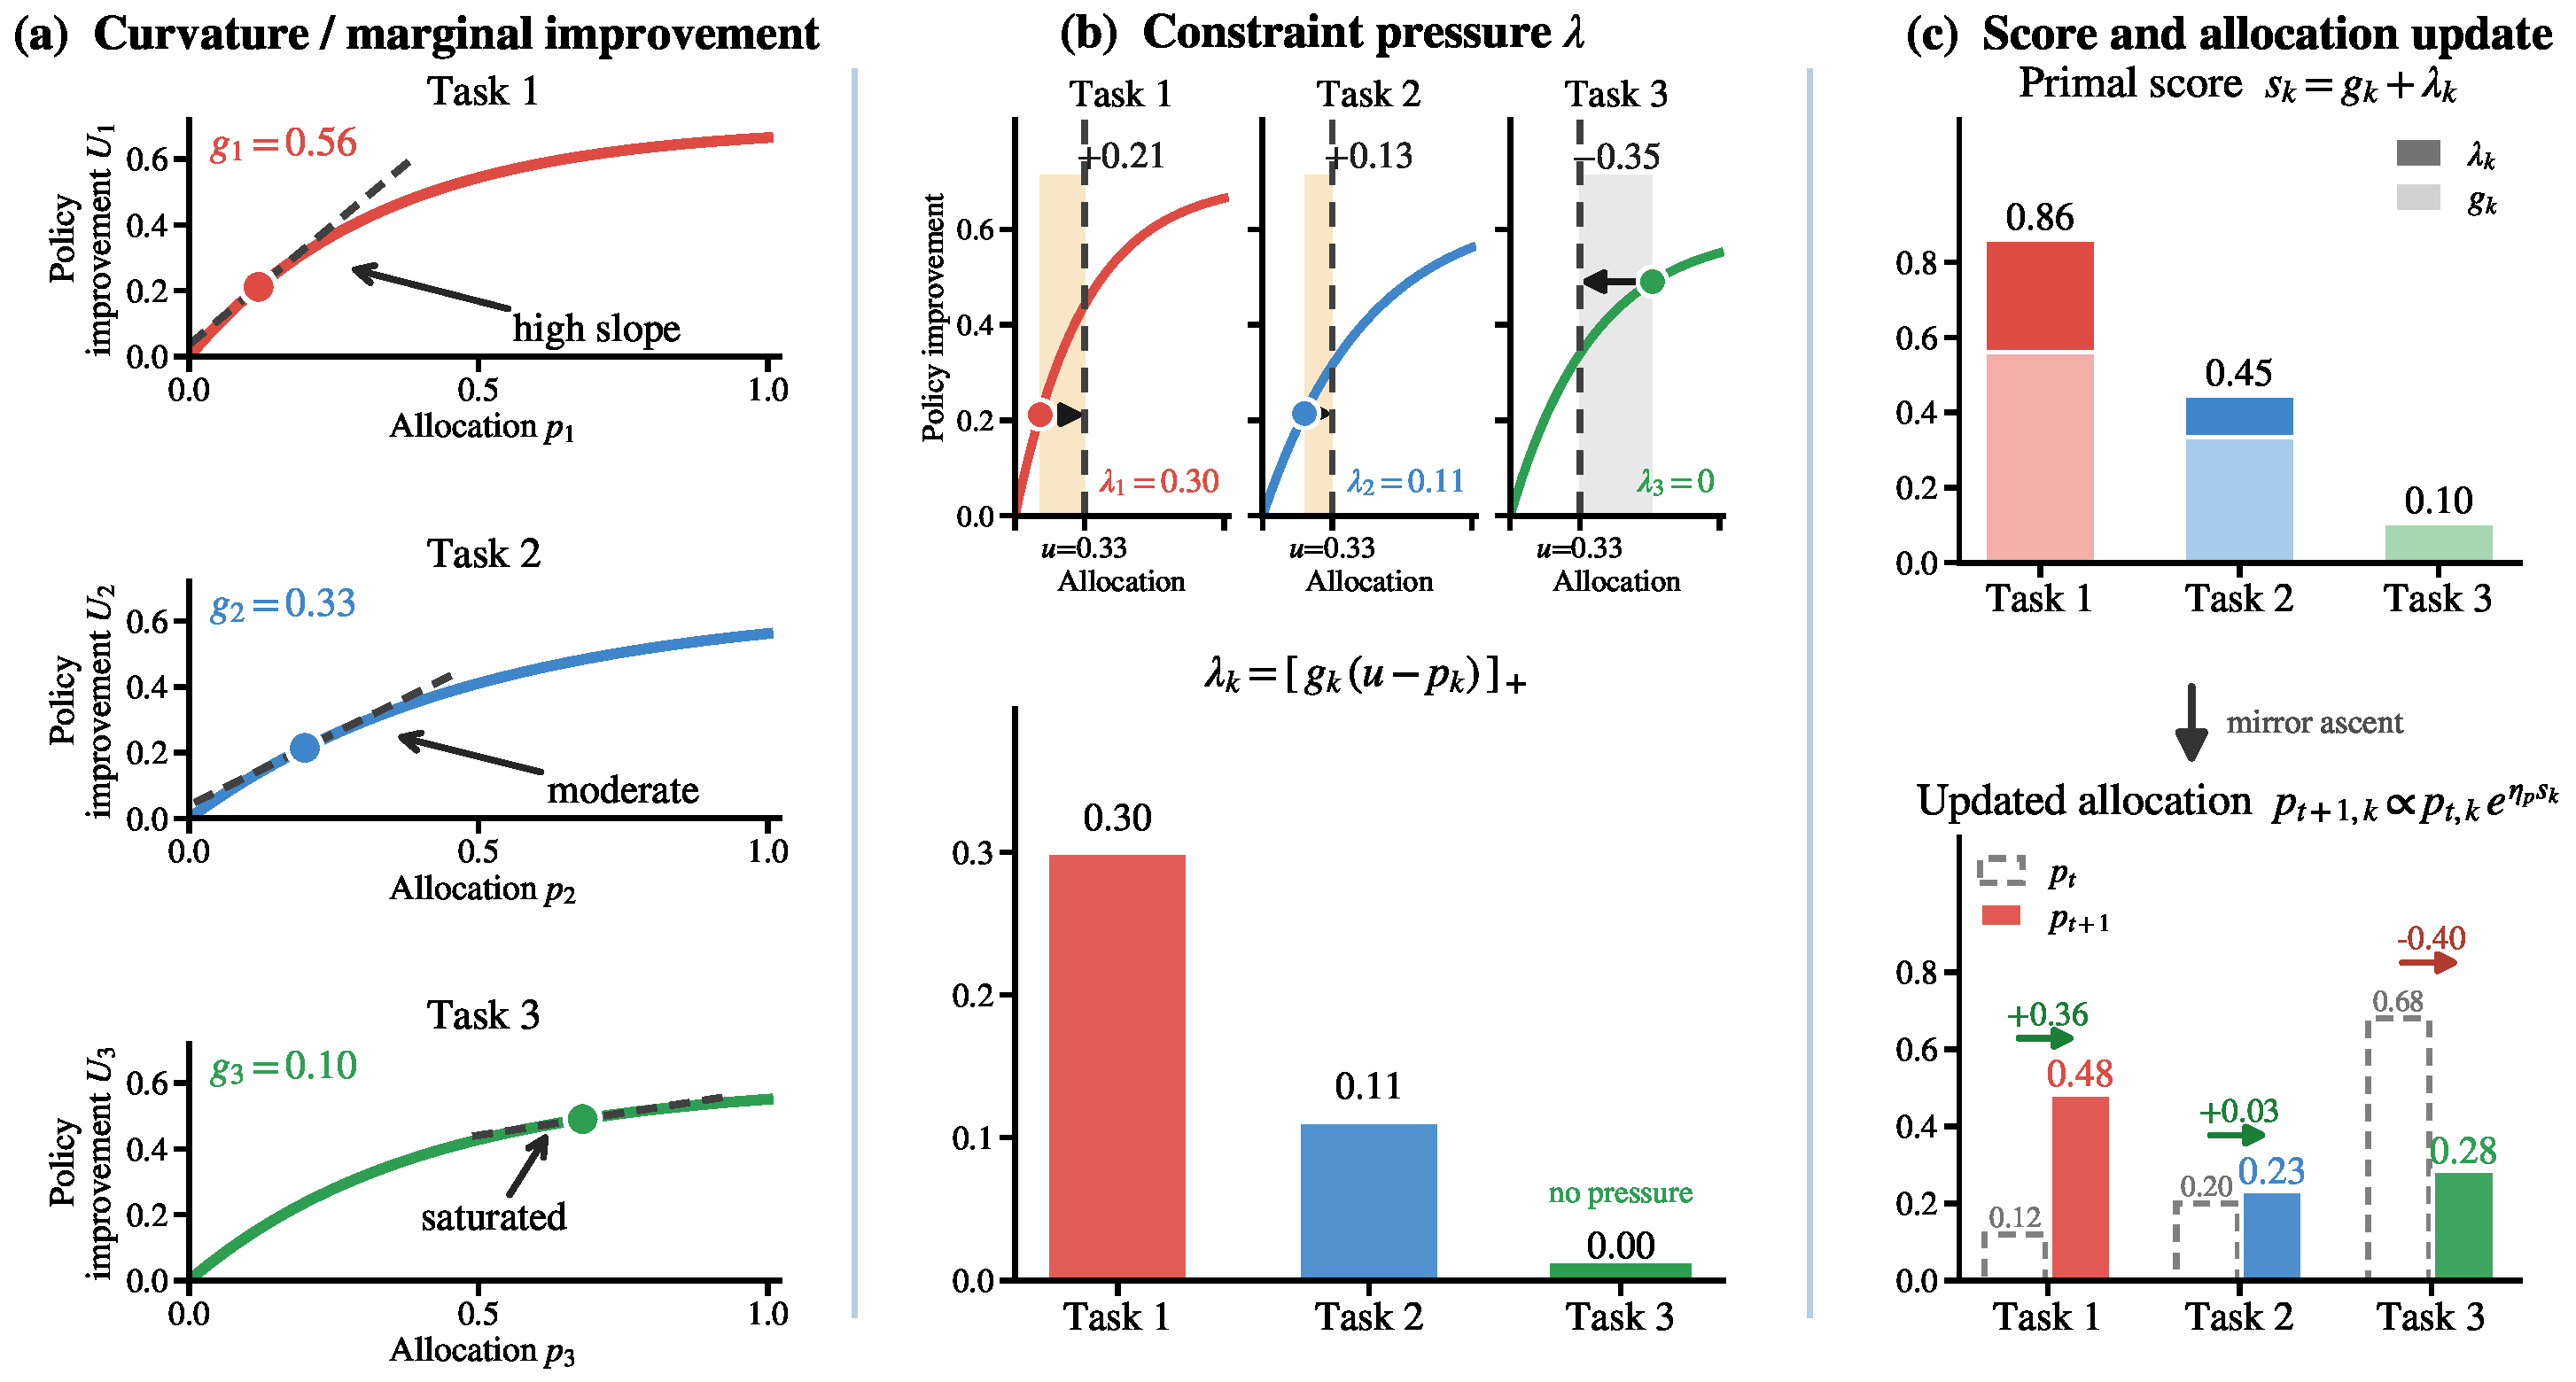
\includegraphics[width=\textwidth]{fig/pdcm_main_fig.pdf}
    \vspace{-\intextsep}
    \caption{%
        \textbf{Curvature-driven allocation in PDCM.}
        \textbf{(a)} Concave policy improvement per task; the slope
        $g_k=\partial U_k/\partial p_k$ at the current allocation gives the marginal
        return (Task~1 steep, Task~3 saturated).
        \textbf{(b)} Constraint pressure as an alignment of the uniform gap with
        curvature, $\lambda_k=[g_k(u-p_k)]_+$, $u=1/K$: only tasks that are both
        under-allocated and still improving accumulate pressure.
        \textbf{(c)} The primal score $s_k=g_k+\lambda_k$ drives the mirror-ascent
        update $p_{t+1,k}\propto p_{t,k}e^{\eta_p s_k}$, moving budget from the
        saturated task to the steep, under-served one.
    }
    \label{fig:pdcm_overview}
    \vspace{-\intextsep}
\end{figure*}

\subsection{Primal-Dual Curvature Matching}
To solve Problem~\labelcref{eq:constrained_optimization_problem}, one must optimize an online objective over the probability simplex while satisfying cumulative constraints. This class of problems has been extensively studied using Primal-Dual Mirror Descent (PDMD)~\citep{Beck2003MirrorDA,mahdavi2011trading,jenatton2015adaptivealgorithmsonlineconvex}. PDMD controls the allocation via an exponential update rule
\begin{equation} \label{eq:primal_update}
p_{t+1,j}
= 
\frac{p_{t,j}\exp(\eta_p s_{t,j})}
{\sum_{\ell=1}^Kp_{t,\ell}\exp(\eta_p s_{t,\ell})},
\end{equation}
where $s_{t,j}$ is the corresponding score of task $j$ at iteration $t$. In a generic PDMD formulation, this score combines the gradient of the primal objective with dual-weighted gradients of the constraints. In Problem~\labelcref{eq:constrained_optimization_problem}, however, the task-wise counterfactual constraints are linearized surrogates of the same task-wise utility functions that define the primal objective. Consequently, the task-wise score $s_{t, j}$ is obtained by amplifying the marginal-utility signal in $g_{t, k}$ according to the current lag pressure encoded by $\lambda_t$.
\begin{equation} \label{eq:dual_weighted_marginal_utility_vectorized}
s_t
=
G_t^\top \left( \mathbf{1} + \lambda_t \right)
\qquad
\text{, where }
G_t
    =
    \begin{bmatrix}
    g_{t,1}^{\top}\\
    \vdots\\
    g_{t,K}^{\top}
    \end{bmatrix}
\end{equation}
The lag pressure $\lambda_t$ is accumulated over iterations through projected dual ascent. Specifically, for each task $k$,
\begin{equation} \label{eq:dual_update}
\lambda_{t+1, k} = \left[ \lambda_{t, k} + \eta_\lambda \left( \langle g_{t, k}, u - p_t \rangle - \epsilon \right) \right]_+,
\end{equation}
where $\eta_\lambda$ is the dual step size and $[\cdot]_+$ denotes the projection onto the non-negative plane. The dual update increases the lag pressure for tasks that are underperforming relative to the imaginery uniform baseline, thereby influencing future allocations to favor those tasks. We dub the resulting algorithm \textbf{\textit{Primal-Dual Curvature Matching}} (PDCM), which is summarized in \Cref{alg:pdcm_jacobian}.

\begin{algorithm}[t]
\caption{Primal--Dual Mirror Descent with Full Jacobian}
\label{alg:pdcm_jacobian}
\begin{algorithmic}[1]
\REQUIRE
Number of tasks $K$; horizon $T$;
primal step size $\eta_p>0$;
dual step size $\eta_\lambda>0$;
constraint budget $\epsilon\ge 0$;
Dithering strength schedule $\{\nu_t\}$, where $\nu_t \in [0, 1]$.
\STATE Initialize $p_1 \gets u$, $\lambda_1 \gets \mathbf{0}$ and initial policy $\pi_0$.
\STATE Maintain a history of size $H$ of task-wise improvement vectors $\{\widehat U_\tau\}_{\tau=t-H}^{t-1}$ and allocation-response Jacobians $\{\widehat G_\tau\}_{\tau=t-H}^{t-1}$ and allocations $\{p_\tau\}_{\tau=t-H}^{t-1}$.

\FOR{$t=1,\ldots,T$}
    \STATE Obtain $\pi_t$ through policy update under allocation $p_{t-1}$. \COMMENT{\textcolor{blue}{RL step.}}
    \STATE Compute the task-wise improvement vector by \Cref{eq:policy_improvement_estimation}.
    \[
    \widehat U_t
    =
    \bigl(
    \widehat U_{t,1},\ldots,\widehat U_{t,K}
    \bigr)^\top.
    \]
    \COMMENT{\textcolor{blue}{Extra forward pass with the updated policy.}}

    \STATE Estimate the Jacobian $\widehat G_t$ by \Cref{eq:theil-sen}. \COMMENT{\textcolor{blue}{Applies Theil-Sen regression to estimate first-order sensitivity.}}

    \STATE Compute the primal scores $s_t$ by \Cref{eq:s_combined}.
    \COMMENT{Combine primal and dual weights.}

    \STATE Update the primal allocation $p_{t+1}$ by entropic mirror ascent using \Cref{eq:primal_update}.  \COMMENT{\textcolor{blue}{Exponential weight update.}}
    \STATE Add Dirchelet noise $\Tilde{p}_t = (1 - \nu)p_t + \nu\alpha,  \quad \text{where } \alpha \sim \mathrm{Dirchelet}(1)$ \label{alg:dirchlet}
    \STATE Update the dual variables $\lambda_{t+1}$ by projected gradient ascent using \Cref{eq:dual_update}.
\ENDFOR
\end{algorithmic}
\end{algorithm}

The adaptive allocation in PDCM is intended to exploit temporal variation in task-wise marginal utility. The following result shows that this adaptivity remains asymptotically competitive with any fixed feasible allocation, including the uniform mixture, while simultaneously controlling cumulative task-wise lag.

\begin{theorem}[Constrained no-regret of PDCM]
\label{thm:pdcm_no_regret}
Suppose that each task-wise utility $U_{t,k}$ is twice-differentiable and Assumption~\ref{asm:concavity} holds. Let
\[
p_T^\star
\in
\arg\max_{p\in\mathcal P_T}
\sum_{t=1}^T U_t(p)
\]
denote the best fixed feasible allocation in hindsight. If
$\eta_p,\eta_\lambda=\Theta(T^{-1/2})$, then PDCM satisfies
\begin{equation}
\sum_{t=1}^T
\left[
\sum_{k=1}^K U_{t,k}(p_T^\star) - \sum_{k=1}^K U_{t,k}(p_t)
\right]
=
O(\sqrt{T}),
\end{equation}
while, for every task $k$,
\begin{equation}
\left[
\sum_{t=1}^T
\left(
U_{t,k}(u)-U_{t,k}(p_t)-\epsilon_{t,k}
\right)
\right]_+
=
O(\sqrt{T}).
\end{equation}
Consequently, both the average regret and the average excess counterfactual lag vanish at rate
$O(T^{-1/2})$.
\end{theorem}

\subsection{Policy Improvement Estimation}
The performance difference lemma formulation of policy improvement in \Cref{eq:policy_improvement_is} provides a convenient way to estimate the task-wise policy improvement $U_{t,k}$ using off-policy evaluation~\citep{ope2000}. Specifically, we use generated rollouts from the training batch to estimate the task-wise policy improvement as
\begin{equation} \label{eq:policy_improvement_estimation}
\widehat U_{t,k}
=
\frac{1}{N_k}\sum_{i=1}^{N_k}
\frac{\pi_{t+1}(y_i\mid x_i)}
{\pi_{t}(y_i\mid x_i)}
A_{\pi_{t}}(y_i\mid x_i),
\end{equation}
where $(x_i, y_i)$ are the $i$-th state-action pair in of task $k$ in the training batch on step $t$. We estimate $A_{\pi_t}$ using the z-score estimator used by group-based RL algorithms such as GRPO~\citep{grpo2024} and GSPO~\citep{gspo2025}.

Compared to the standard RL post-training loop, this estimation only requires an additional forward pass of the improved policy $\pi_{t+1}$ to compute the importance sampling ratio $\frac{\pi_{t+1}(y_i\mid x_i)}{\pi_{t}(y_i\mid x_i)}$. This is a negligible overhead compared to the cost of rollout generation or backpropagation.

\subsection{Curvature Estimation}
What is left is to estimate the allocation-response Jacobian $g_{t, k}$. Estimating such quantity also requires a counterfactual evaluation of the policy improvement around $p_t$. However, by maintaining a history of task-wise improvement vectors $\{\widehat U_\tau\}_{\tau=1}^{t-1}$ and allocations $\{p_\tau\}_{\tau=1}^{t-1}$, we can approximate the allocation-response Jacobian $g_{t, k}$ by local regression. We opt for Theil-Sen estimator~\citep{Theil1992} for its robustness to noisy performance difference estimates $\hat{U}_{t, k}$ when the allocation $p_{t, k}$ is low.
\begin{equation} \label{eq:theil-sen}
\widehat g_{t,kj}
=
\operatorname*{median}_{\substack{1\le a<b\le t-1\\ |p_{b,j}-p_{a,j}|>\delta}}
\frac{\widehat U_{b,k}-\widehat U_{a,k}}{p_{b,j}-p_{a,j}} .
\qquad
\forall k\in[K], j\in[K].
\end{equation}

